\documentclass{standalone}
\usepackage{graphicx}	
\usepackage{amssymb, amsmath}
\usepackage{color}

\usepackage{tikz}
\usetikzlibrary{calc, arrows.meta}
\usepackage{pgfmath}

\definecolor{light}{RGB}{220, 188, 188}
\definecolor{mid}{RGB}{185, 124, 124}
\definecolor{dark}{RGB}{143, 39, 39}
\definecolor{highlight}{RGB}{180, 31, 180}
\definecolor{gray10}{gray}{0.1}
\definecolor{gray20}{gray}{0.2}
\definecolor{gray30}{gray}{0.3}
\definecolor{gray40}{gray}{0.4}
\definecolor{gray60}{gray}{0.6}
\definecolor{gray70}{gray}{0.7}
\definecolor{gray80}{gray}{0.8}
\definecolor{gray90}{gray}{0.9}
\definecolor{gray95}{gray}{0.95}

\newcommand*{\offset}{0.025}

\begin{document}

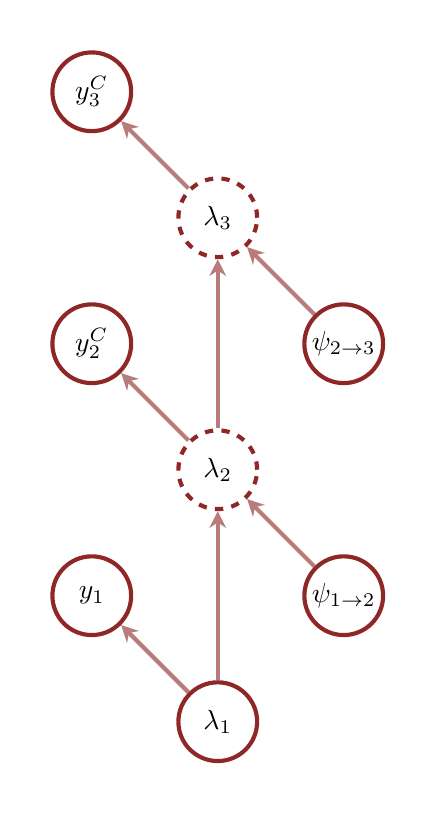
\begin{tikzpicture}[scale=0.2, thick]

  \pgfmathsetmacro{\r}{2.5}
    
  \draw[white] (-12, -4) rectangle (12, 44);

  \coordinate (A) at (0, 0);
  \coordinate (B) at (0, 16);
  \coordinate (C) at (0, 32);

  \coordinate (D) at (8, 8);
  \coordinate (E) at (8, 24);

  \coordinate (F) at (-8, 8);
  \coordinate (G) at (-8, 24);
  \coordinate (H) at (-8, 40);

  \coordinate (I) at (-8, 18);
  \coordinate (J) at (-8, 34);

  \coordinate (K) at (-16, 16);
  \coordinate (L) at (-16, 32);
  
  \foreach \B/\E in {A/B, A/F, D/B, B/C, B/G, E/C, C/H} {
    \draw[-{Stealth[length=6pt, width=6pt]}, shorten <=15, shorten >=15, color=mid, line width=1.5] (\B) -- (\E);
  }

  \filldraw[fill=white, draw=dark, line width=1.5] (A) circle (\r)
  node[color=black] { $\lambda_{1}$ };

  \filldraw[fill=white, draw=dark, dashed, line width=1.5] (B) circle (\r)
  node[color=black] { $\lambda_{2}$ };
  
  \filldraw[fill=white, draw=dark, dashed, line width=1.5] (C) circle (\r)
  node[color=black] { $\lambda_{3}$ };

  \filldraw[fill=white, draw=dark, line width=1.5] (D) circle (\r)
  node[color=black] { $\psi_{1 \rightarrow 2}$ };
  
  \filldraw[fill=white, draw=dark, line width=1.5] (E) circle (\r)
  node[color=black] { $\psi_{2 \rightarrow 3}$ };

  \filldraw[fill=white, draw=dark, line width=1.5] (F) circle (\r)
  node[color=black] { $y_{1}$ };
  
  \filldraw[fill=white, draw=dark, line width=1.5] (G) circle (\r)
  node[color=black] { $y_{2}^{C}$ };
  
  \filldraw[fill=white, draw=dark, line width=1.5] (H) circle (\r)
  node[color=black] { $y_{3}^{C}$ };

\end{tikzpicture}

\end{document}  